% Created 2024-02-14 Wed 13:38
% Intended LaTeX compiler: xelatex
\documentclass[presentation, aspectratio=1610]{beamer}
\usepackage{graphicx}
\usepackage{longtable}
\usepackage{wrapfig}
\usepackage{rotating}
\usepackage[normalem]{ulem}
\usepackage{capt-of}
\usepackage{hyperref}
\definecolor{UFBLUE}{HTML}{5d89cb}
\setbeamercolor{frametitle}{bg=UFBLUE}
\usepackage{graphicx}
\usetheme[progressbar=foot]{metropolis}
\usepackage[sorting=ynt,backend=biber,style=ieee]{biblatex}
\addbibresource{../src/myBib.bib}
\usepackage{threeparttable}
\usepackage{multirow}
\usepackage{tabularx}
\renewcommand*{\bibfont}{\scriptsize}
\usepackage{caption}
\captionsetup[figure]{labelformat=empty}
\DeclareMathOperator*{\argmax}{\arg\!max}
\DeclareMathOperator*{\argmin}{\arg\!min}
\AtBeginSubsection{\begin{frame}\tableofcontents[currentsection,currentsubsection]\end{frame}}
\usepackage{tcolorbox}
\tcbuselibrary{fitting}
\usetheme{metropolis}
\usecolortheme{}
\usefonttheme{}
\useinnertheme{}
\useoutertheme{}
\author{Andrew Jensen}
\date{March 4, 2024}
\title{Methods for Autonomous Measurement of 3D Joint Kinematics from 2D Fluoroscopic Images}
\subtitle{A Dissertation Defense}
\hypersetup{
 pdfauthor={Andrew Jensen},
 pdftitle={Methods for Autonomous Measurement of 3D Joint Kinematics from 2D Fluoroscopic Images},
 pdfkeywords={},
 pdfsubject={},
 pdfcreator={Emacs 29.2 (Org mode 9.7)}, 
 pdflang={English}}
\begin{document}

\maketitle
\begin{frame}{Outline}
\tableofcontents
\end{frame}

\begin{frame}[label={sec:org9e76876}]{Acknowledgments}
I would like to thank the McJunkin Family Charitable Foundation for their generous grant that supports this work.
\end{frame}
\begin{frame}[label={sec:org9ac33c4}]{The Problem}
\begin{columns}
\begin{column}{0.5\columnwidth}
\begin{itemize}
\item By 2030, roughly 3.5 million Total Knee Arthroplasty (TKA) will be performed in the US \autocite{kurtzProjectionsPrimaryRevision2007}.
\item 20\% of patients receiving TKA are dissatisfied.
\begin{itemize}
\item Instability, pain, unnatural \autocites{bakerRolePainFunction2007}[][]{bournePatientSatisfactionTotal2010}[][]{scottPredictingDissatisfactionFollowing2010}.
\end{itemize}
\item No reliable method of clinically assessing and quantifying joint dynamics.
\begin{itemize}
\item Human supervision
\item Time consuming
\item Specialized equipment
\end{itemize}
\end{itemize}
\end{column}
\begin{column}{0.5\columnwidth}
\begin{center}
\includegraphics[width=\textwidth]{/home/ajensen123@ad.ufl.edu/repo/lit-review/figures/raster/Physical_Examination_of_the_knee.jpg}
\end{center}
\end{column}
\end{columns}
\end{frame}
\begin{frame}[label={sec:org25dba94}]{Our Proposition}
\begin{columns}
\begin{column}{0.5\columnwidth}
Orthopaedic surgeons and clinicians would readily adopt a \alert{\alert{practical}} and \alert{\alert{inexpensive}} technology that allows them to \alert{\alert{measure}} a patient's knee kinematics during \alert{\alert{activities of daily living}}.
\end{column}
\begin{column}{0.55\columnwidth}
\begin{center}
\includegraphics[width=2in]{/home/ajensen123@ad.ufl.edu/repo/lit-review/figures/raster/dynamic-knee-prescription.png}
\end{center}
\end{column}
\end{columns}
\end{frame}
\begin{frame}[label={sec:org9503eea}]{Constraints}
\begin{columns}
\begin{column}{0.45\columnwidth}
\begin{itemize}
\item It must fit within a \alert{\alert{standard clinical workflow}}
\item The technology must utilize equipment \alert{\alert{commonly found in hospitals}}
\item There must not be significant \alert{\alert{human supervision}} nor interaction to generate an examination report.
\end{itemize}
\end{column}
\begin{column}{0.55\columnwidth}
\begin{center}
\includegraphics[width=\textwidth]{/home/ajensen123@ad.ufl.edu/repo/lit-review/figures/raster/c-arm-fluoro-machine.jpg}
\end{center}
\end{column}
\end{columns}
\end{frame}
\section{Background}
\label{sec:org2262a80}
\begin{frame}[label={sec:orge79ba77}]{Background - Projective Geometry}
\begin{center}
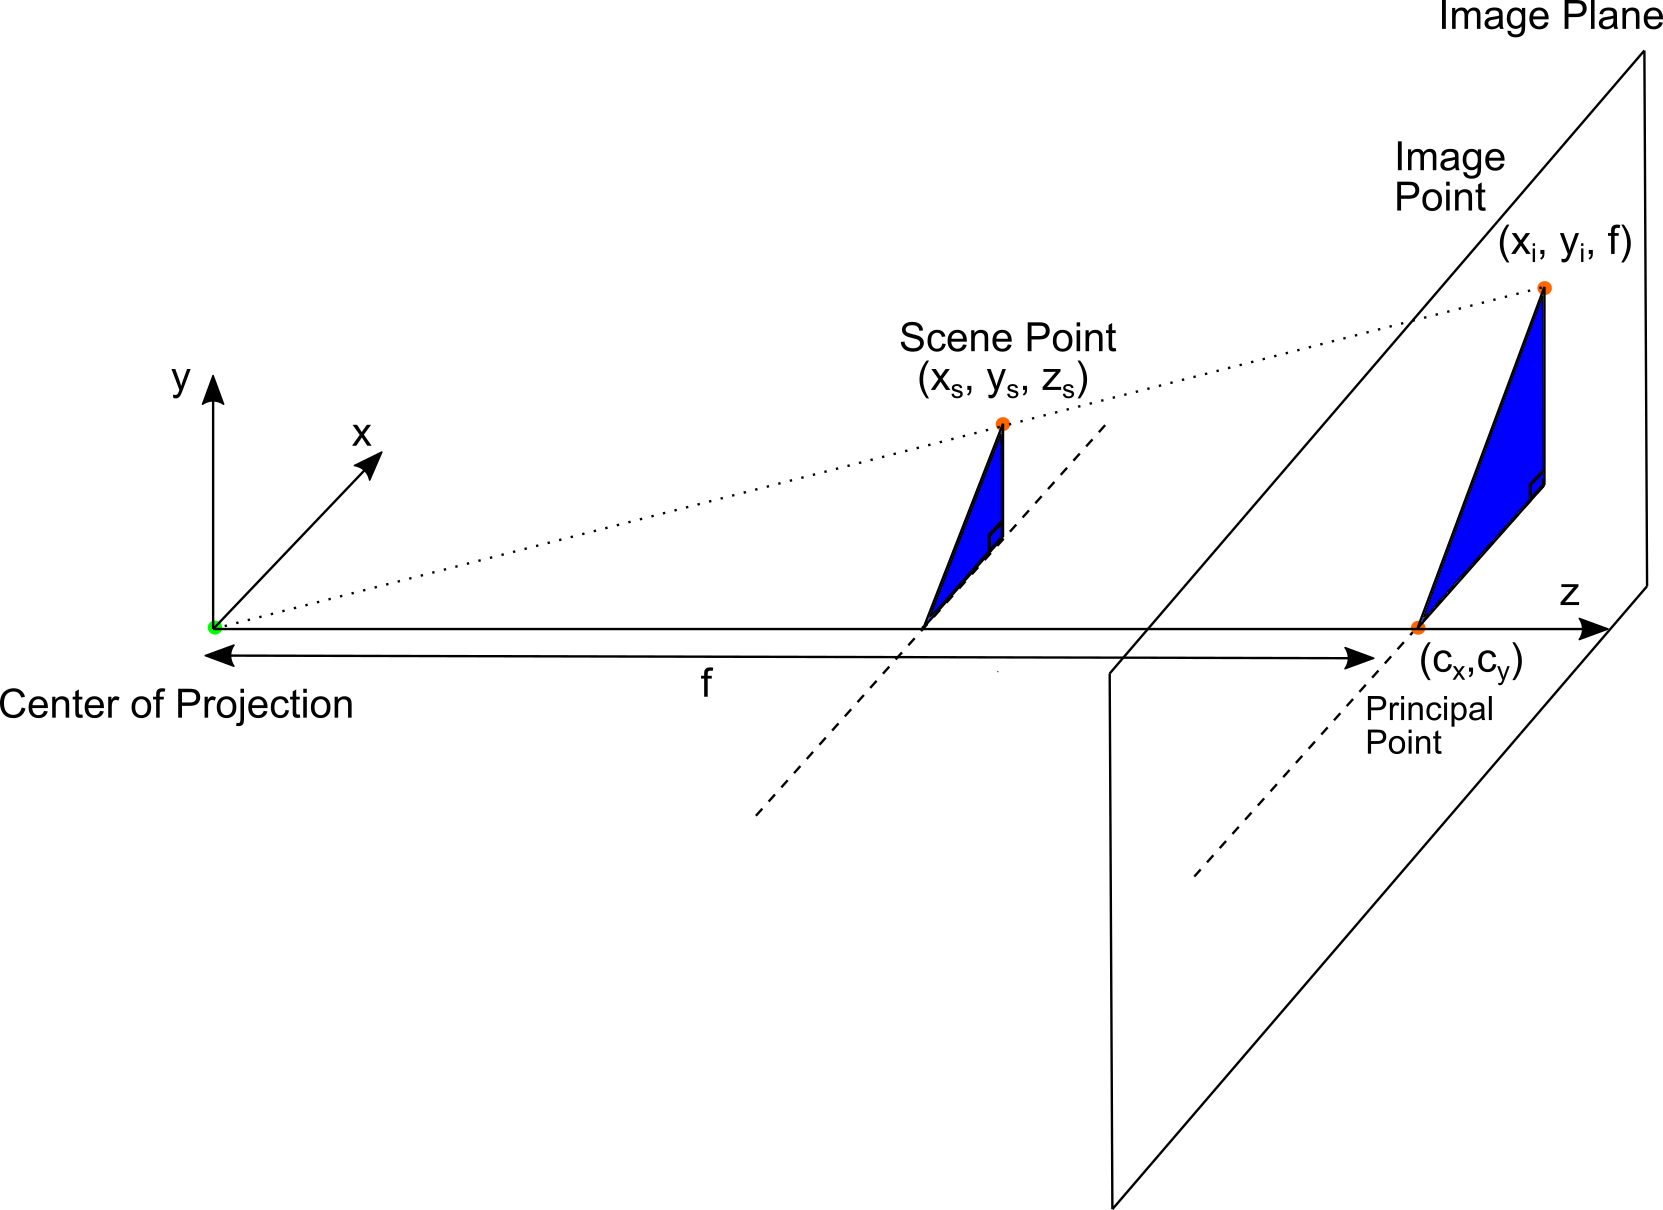
\includegraphics[width=0.8\textwidth]{/home/ajensen123@ad.ufl.edu/repo/lit-review/figures/raster/perspective-projection.png}
\end{center}
\end{frame}
\begin{frame}[label={sec:org2ff9234}]{Background - Model-Image Registration}
\begin{columns}
\begin{column}{0.5\columnwidth}
If we know the projective parameters of the fluoroscopy machine, can we tinker with \(T^{cam}_{implant}\) so that our virtual projection matches the fluoroscopic image?
\end{column}
\begin{column}{0.6\columnwidth}
\begin{figure}[htbp]
\centering
\includegraphics[width=2.5in]{/home/ajensen123@ad.ufl.edu/repo/lit-review/figures/raster/registered-tka.png}
\caption{From \autocite{mahfouzRobustMethodRegistration2003}}
\end{figure}
\end{column}
\end{columns}
\end{frame}
\begin{frame}[label={sec:orgc3e0df4}]{Background - Model-Image Registration}
\begin{columns}
\begin{column}{0.5\columnwidth}
If we know the projective parameters of the fluoroscopy machine, can we tinker with \(T^{cam}_{implant}\) so that our virtual projection matches the fluoroscopic image?
\end{column}
\begin{column}{0.6\columnwidth}
\begin{figure}[htbp]
\centering
\includegraphics[width=2.5in]{/home/ajensen123@ad.ufl.edu/repo/lit-review/figures/raster/mahfouz-perspective-projection.png}
\caption{From \autocite{mahfouzRobustMethodRegistration2003}}
\end{figure}
\end{column}
\end{columns}
\end{frame}
\begin{frame}[label={sec:org4448662}]{Historical Overview}
Many different approaches have attempted to solve the model-image registration problem.
\begin{itemize}
\item Pre-computed projections
\item Skin-mounted motion Capture
\item Biplane Imaging
\item Iterative Projections
\item Roentgen Stereophotogrammetry
\end{itemize}
\end{frame}
\begin{frame}[label={sec:orga114031}]{Pre-Computed Projections}
\begin{columns}
\begin{column}{0.5\columnwidth}
\begin{itemize}
\item Saving space and memory by pre-computing as much as possible.
\item Pre-computed distance maps \autocites{zuffiModelbasedMethodReconstruction1999}[][]{lavalleeRecoveringPositionOrientation1995}.
\item Pre-computed shape libraries \autocite{banksAccurateMeasurementThreedimensional1996}
\end{itemize}
\end{column}
\begin{column}{0.6\columnwidth}
\begin{figure}[htbp]
\centering
\includegraphics[width=1.75in]{/home/ajensen123@ad.ufl.edu/repo/lit-review/figures/raster/lavallee-distance-maps.png}
\caption{From \autocite{lavalleeRecoveringPositionOrientation1995}}
\end{figure}
\begin{figure}[htbp]
\centering
\includegraphics[width=1.75in]{/home/ajensen123@ad.ufl.edu/repo/lit-review/figures/raster/banks-nfd-library.png}
\caption{From \autocite{banksAccurateMeasurementThreedimensional1996}}
\end{figure}
\end{column}
\end{columns}
\end{frame}
\begin{frame}[label={sec:orgf2926e7}]{Limitations of Pre-Computed Projections}
\begin{columns}
\begin{column}{0.5\columnwidth}
\begin{itemize}
\item Requires an accurate contour from the input image in order to perform calculations.
\begin{itemize}
\item Human supervision for isolated contour
\item Inaccuaracy with naive edge detection
\end{itemize}
\end{itemize}
\end{column}
\begin{column}{0.6\columnwidth}
\begin{figure}[htbp]
\centering
\includegraphics[width=1.75in]{/home/ajensen123@ad.ufl.edu/repo/lit-review/figures/raster/lavallee-distance-maps.png}
\caption{From \autocite{lavalleeRecoveringPositionOrientation1995}}
\end{figure}
\begin{figure}[htbp]
\centering
\includegraphics[width=1.75in]{/home/ajensen123@ad.ufl.edu/repo/lit-review/figures/raster/banks-nfd-library.png}
\caption{From \autocite{banksAccurateMeasurementThreedimensional1996}}
\end{figure}
\end{column}
\end{columns}
\end{frame}
\begin{frame}[label={sec:orge48eec9}]{Motion Capture (MoCap)}
\begin{columns}
\begin{column}{0.5\columnwidth}
\begin{itemize}
\item Can measure motion of MoCap beads very accurately.
\item Skin-mounted \autocites{gaoInvestigationSoftTissue2008}[][]{kuoInfluenceSoftTissue2011}[][]{linEffectsSoftTissue2016}.
\item Bone pins \autocite{lafortuneThreedimensionalKinematicsHuman1992}.
\end{itemize}
\end{column}
\begin{column}{0.6\columnwidth}
\begin{figure}[htbp]
\centering
\includegraphics[width=2.5in]{/home/ajensen123@ad.ufl.edu/repo/lit-review/figures/raster/gao-skin-mocap.png}
\caption{From \autocite{gaoInvestigationSoftTissue2008}}
\end{figure}
\begin{figure}[htbp]
\centering
\includegraphics[width=2.5in]{/home/ajensen123@ad.ufl.edu/repo/lit-review/figures/raster/lafortune-bone-mocap.png}
\caption{From \autocite{lafortuneThreedimensionalKinematicsHuman1992}}
\end{figure}
\end{column}
\end{columns}
\end{frame}
\begin{frame}[label={sec:org0d6f04a}]{Limitations of Motion Capture}
\begin{columns}
\begin{column}{0.5\columnwidth}
Skin Mounted
\begin{itemize}
\item Doesn't accurately describe underlying skeletal motion with clinical accuracy \autocites{gaoInvestigationSoftTissue2008}[][]{kuoInfluenceSoftTissue2011}[][]{linEffectsSoftTissue2016}.
\end{itemize}
Bone Pins
\begin{itemize}
\item Any volunteers?
\end{itemize}
\end{column}
\begin{column}{0.6\columnwidth}
\begin{figure}[htbp]
\centering
\includegraphics[width=2.5in]{/home/ajensen123@ad.ufl.edu/repo/lit-review/figures/raster/gao-skin-mocap.png}
\caption{From \autocite{gaoInvestigationSoftTissue2008}}
\end{figure}
\begin{figure}[htbp]
\centering
\includegraphics[width=2.5in]{/home/ajensen123@ad.ufl.edu/repo/lit-review/figures/raster/lafortune-bone-mocap.png}
\caption{From \autocite{lafortuneThreedimensionalKinematicsHuman1992}}
\end{figure}
\end{column}
\end{columns}
\end{frame}
\begin{frame}[label={sec:org3b91854}]{Biplane Imaging}
\begin{columns}
\begin{column}{0.5\columnwidth}
\begin{itemize}
\item Utilizes multiple cameras to resolve 3D position and orientation\autocites{ivesterReconfigurableHighSpeedStereoRadiography2015}[][]{burtonAutomaticTrackingHealthy2021}.
\begin{itemize}
\item Highly accurate.
\item Gold Standard.
\end{itemize}
\end{itemize}
\end{column}
\begin{column}{0.6\columnwidth}
\begin{figure}[htbp]
\centering
\includegraphics[width=1.75in]{/home/ajensen123@ad.ufl.edu/repo/lit-review/figures/raster/ivester-stereo-fluoromachine.png}
\caption{Both from \autocite{ivesterReconfigurableHighSpeedStereoRadiography2015}}
\end{figure}
\begin{figure}[htbp]
\centering
\includegraphics[width=1.75in]{/home/ajensen123@ad.ufl.edu/repo/lit-review/figures/raster/ivester-stereo-projection.png}
\end{figure}
\end{column}
\end{columns}
\end{frame}
\begin{frame}[label={sec:org1a3fe08}]{Limitations of Biplane Imaging}
\begin{columns}
\begin{column}{0.5\columnwidth}
\begin{itemize}
\item Not many hospitals have biplane fluoroscopy setups.
\item Clinically impractical
\end{itemize}
\end{column}
\begin{column}{0.6\columnwidth}
\begin{figure}[htbp]
\centering
\includegraphics[width=1.75in]{/home/ajensen123@ad.ufl.edu/repo/lit-review/figures/raster/ivester-stereo-fluoromachine.png}
\caption{Both from \autocite{ivesterReconfigurableHighSpeedStereoRadiography2015}}
\end{figure}
\begin{figure}[htbp]
\centering
\includegraphics[width=1.75in]{/home/ajensen123@ad.ufl.edu/repo/lit-review/figures/raster/ivester-stereo-projection.png}
\end{figure}
\end{column}
\end{columns}
\end{frame}
\begin{frame}[label={sec:org6bb6e57}]{Iterative Projections}
\begin{columns}
\begin{column}{0.54\columnwidth}
\begin{itemize}
\item Take advantage of modern computational graphics pipelines to quickly perform projection matching.
\begin{itemize}
\item Image/Intensity similarity metrics \autocite{mahfouzRobustMethodRegistration2003}
\item Feature/Contour similarity metrics \autocite{floodAutomatedRegistration3D2018}
\end{itemize}
\end{itemize}
\end{column}
\begin{column}{0.6\columnwidth}
\begin{figure}[htbp]
\centering
\includegraphics[width=2in]{/home/ajensen123@ad.ufl.edu/repo/lit-review/figures/raster/mahfouz-perspective-projection.png}
\caption{From \autocite{mahfouzRobustMethodRegistration2003}}
\end{figure}
\begin{figure}[htbp]
\centering
\includegraphics[width=2in]{/home/ajensen123@ad.ufl.edu/repo/lit-review/figures/raster/flood-dilated-contour.png}
\caption{From \autocite{floodAutomatedRegistration3D2018}}
\end{figure}
\end{column}
\end{columns}
\end{frame}
\begin{frame}[label={sec:org7de3f80}]{Limitations of (historic) Iterative Projection Methods}
\begin{columns}
\begin{column}{0.54\columnwidth}
\begin{itemize}
\item Requires human supervision for:
\begin{itemize}
\item Pose initialization
\item Escaping local minima
\item Implant detection
\end{itemize}
\item Chaotic and Noisy objective function
\end{itemize}
\end{column}
\begin{column}{0.6\columnwidth}
\begin{figure}[htbp]
\centering
\includegraphics[width=2in]{/home/ajensen123@ad.ufl.edu/repo/lit-review/figures/raster/mahfouz-perspective-projection.png}
\caption{From \autocite{mahfouzRobustMethodRegistration2003}}
\end{figure}
\begin{figure}[htbp]
\centering
\includegraphics[width=2in]{/home/ajensen123@ad.ufl.edu/repo/lit-review/figures/raster/flood-dilated-contour.png}
\caption{From \autocite{floodAutomatedRegistration3D2018}}
\end{figure}
\end{column}
\end{columns}
\end{frame}
\begin{frame}[label={sec:org72a0dc8}]{Roentgen Stereophotogrammetry (RSA)}
\begin{columns}
\begin{column}{0.5\columnwidth}
\begin{itemize}
\item Uses implanted tantalum beads for motion tracking \autocites{vroomanFastAccurateAutomated1998}[][]{selvikRoentgenStereophotogrammetryMethod1989}
\item Extremely accurate \autocites{kapteinEvaluationThreePose2004}[][]{saariKneeKinematicsMedial2005}
\item Gold standard Measurement \autocite{brobergValidationMachineLearning2023}
\end{itemize}
\end{column}
\begin{column}{0.6\columnwidth}
\begin{figure}[htbp]
\centering
\includegraphics[width=3in]{/home/ajensen123@ad.ufl.edu/repo/lit-review/figures/raster/vrooman-mbrsa.png}
\caption{From \autocite{vroomanFastAccurateAutomated1998}}
\end{figure}
\end{column}
\end{columns}
\end{frame}
\begin{frame}[label={sec:org41f5b23}]{Limitations of RSA}
\begin{columns}
\begin{column}{0.5\columnwidth}
\begin{itemize}
\item Involves additional surgical procedures for inserting tantalum beads.
\item Human supervision
\item Bi-plane imaging
\end{itemize}
\end{column}
\begin{column}{0.6\columnwidth}
\begin{figure}[htbp]
\centering
\includegraphics[width=3in]{/home/ajensen123@ad.ufl.edu/repo/lit-review/figures/raster/vrooman-mbrsa.png}
\caption{From \autocite{vroomanFastAccurateAutomated1998}}
\end{figure}
\end{column}
\end{columns}
\end{frame}
\section{Aims}
\label{sec:org39f746e}
\begin{frame}[label={sec:org5d2737a}]{Aims}
\alert{Aim 1:} Joint Track Machine Learning: An Autonomous Method of Measuring Total Knee Arthroplasty Kinematics From Single-Plane X-Ray Images\footnote{Published in the Journal of Arthroplasty \autocite{jensenJointTrackMachine2023}}
\vfill
\alert{Aim 2:} Correcting Symmetric Implant Ambiguity in Measuring Total Knee Arthroplasty Kinematics from Single-Plane Fluoroscopy \footnote{In Revision for Publication in the Journal of Biomechanics}
\vfill
\alert{Aim 3:} Some Musings on a ``Kinematics Translator'' and Synthetic Kinematcs Data
\vfill
\alert{Aim 4:} This will definitely work on shoulders, right?\footnote{In Review for Publication in the Journal of Computers in Biology and Medicine}
\end{frame}
\subsection{Aim 1 - Joint Track Machine Learning}
\label{sec:org8299059}
\begin{frame}[label={sec:org87d97c8}]{Goal}
Demonstrate the feasibility of a fully autonomous, model-image registration pipeline.
\end{frame}
\begin{frame}[label={sec:org3513cd3}]{Method}
\begin{itemize}
\item Three-tiered approach
\begin{itemize}
\item Convolutional Neural networks (CNN) for autonomous implant detection
\item Normalized Fourier Descriptor shape libraries
\item Robust contour-based global optimization scheme
\end{itemize}
\end{itemize}
\begin{center}
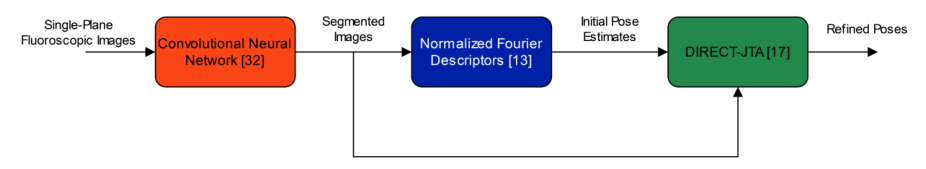
\includegraphics[width=\textwidth]{/home/ajensen123@ad.ufl.edu/repo/lit-review/figures/raster/jtml-pipeline.png}
\end{center}
\end{frame}
\begin{frame}[label={sec:orgf12229e}]{Autonomous Implant Detection Using Convolutional Neural Networks}
\begin{columns}
\begin{column}{0.5\columnwidth}
\begin{itemize}
\item 2 CNNs
\begin{itemize}
\item Femoral and Tibial implants
\end{itemize}
\item High Resolution Network \autocite{wangDeepHighResolutionRepresentation2020}
\end{itemize}
\end{column}
\begin{column}{0.5\columnwidth}
\begin{center}
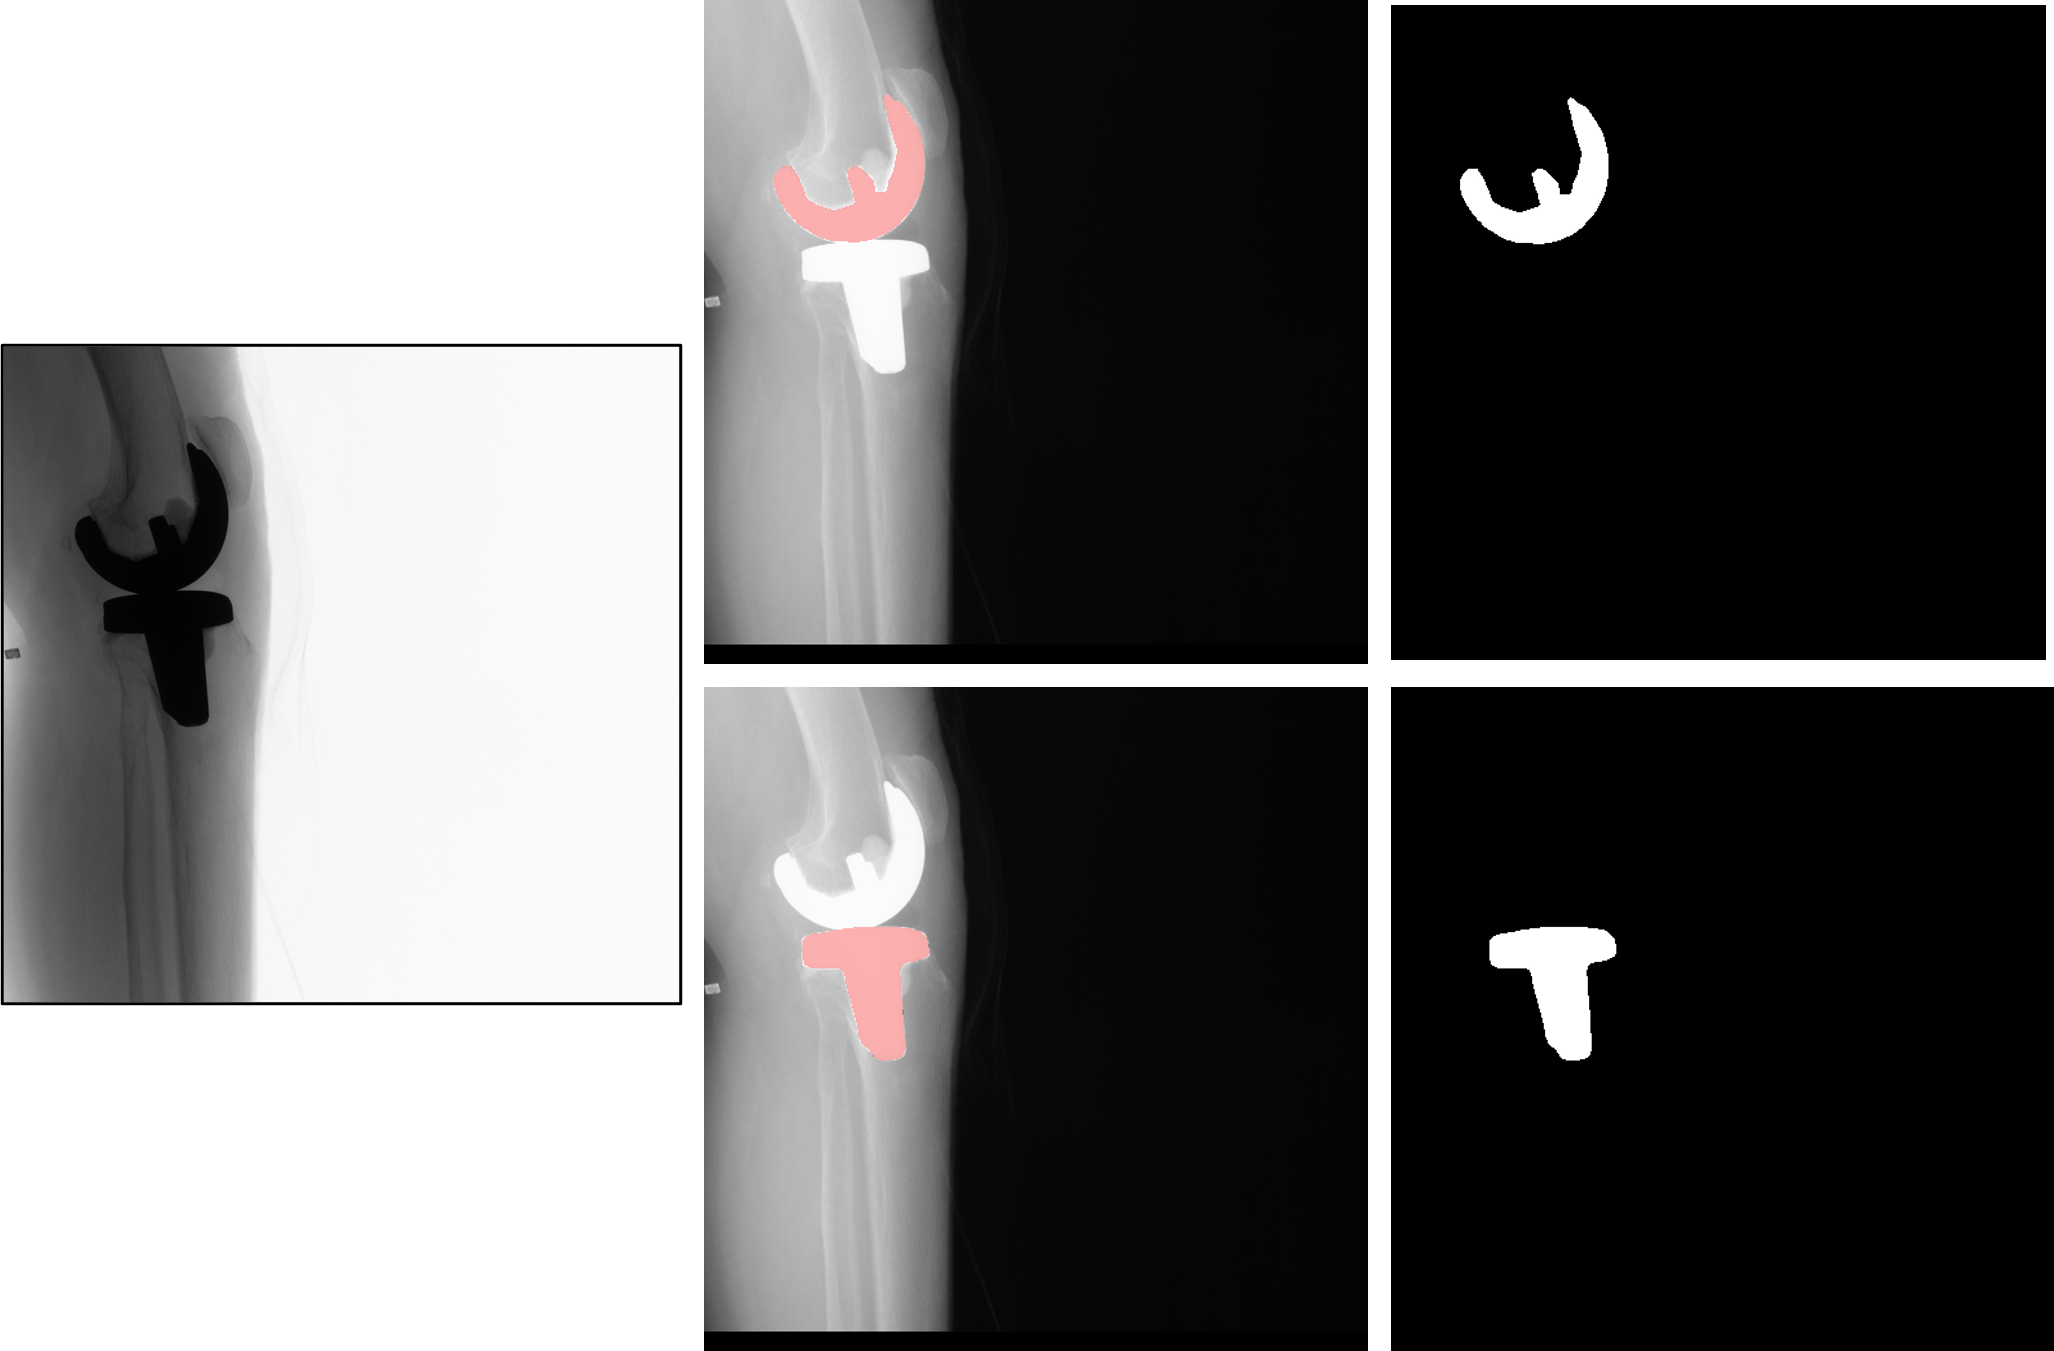
\includegraphics[width=\columnwidth]{/home/ajensen123@ad.ufl.edu/repo/lit-review/figures/raster/jtml-segmentation.png}
\end{center}
\end{column}
\end{columns}
\end{frame}
\begin{frame}[label={sec:orgb0da27b}]{Neural Network Data}
\begin{columns}
\begin{column}{0.5\columnwidth}
\begin{itemize}
\item \textasciitilde{}8000 images
\begin{itemize}
\item 7 TKA kinematics studies
\begin{itemize}
\item 71 subjects
\item 7 implant manufacturers
\item 36 distinct implants
\item Squat, lunge, kneel, stair ascent
\end{itemize}
\end{itemize}
\end{itemize}
\end{column}
\begin{column}{0.6\columnwidth}
\begin{center}
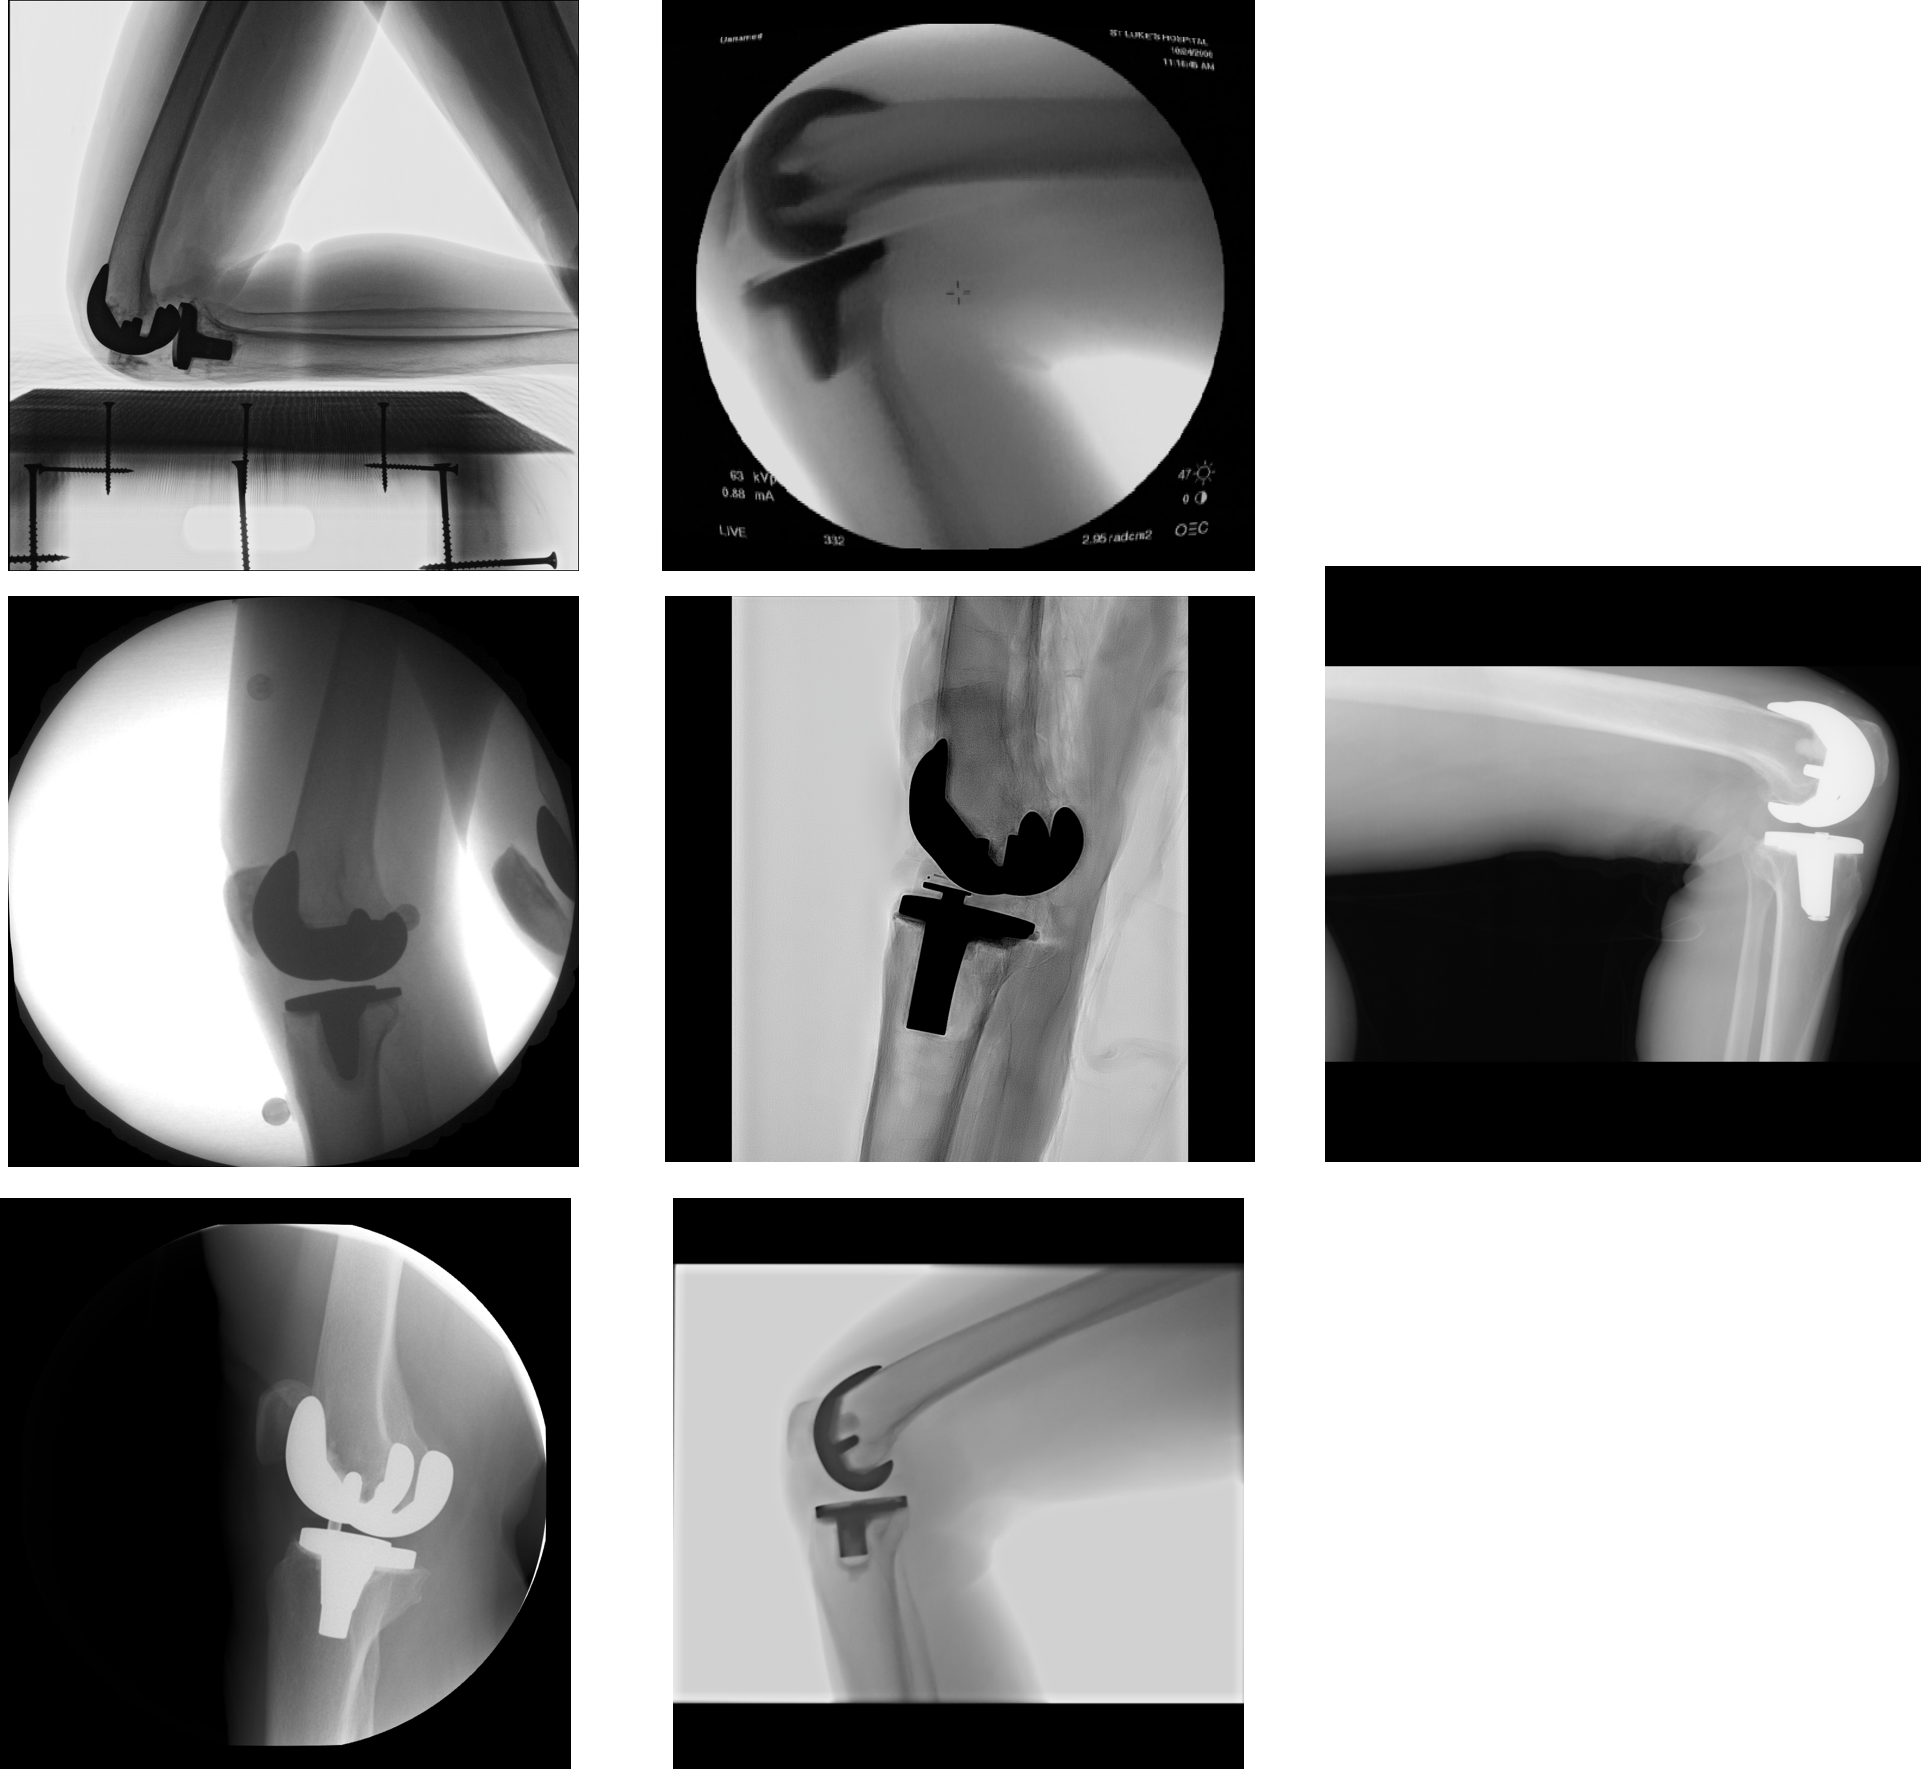
\includegraphics[height=3in]{/home/ajensen123@ad.ufl.edu/repo/lit-review/figures/raster/jtml-data.png}
\end{center}
\end{column}
\end{columns}
\end{frame}
\begin{frame}[label={sec:orgd99f2be}]{Neural Network Robustness}
\begin{itemize}
\item Additional augmentations introduced during training \autocite{buslaevAlbumentationsFastFlexible2020}.
\end{itemize}
\begin{center}
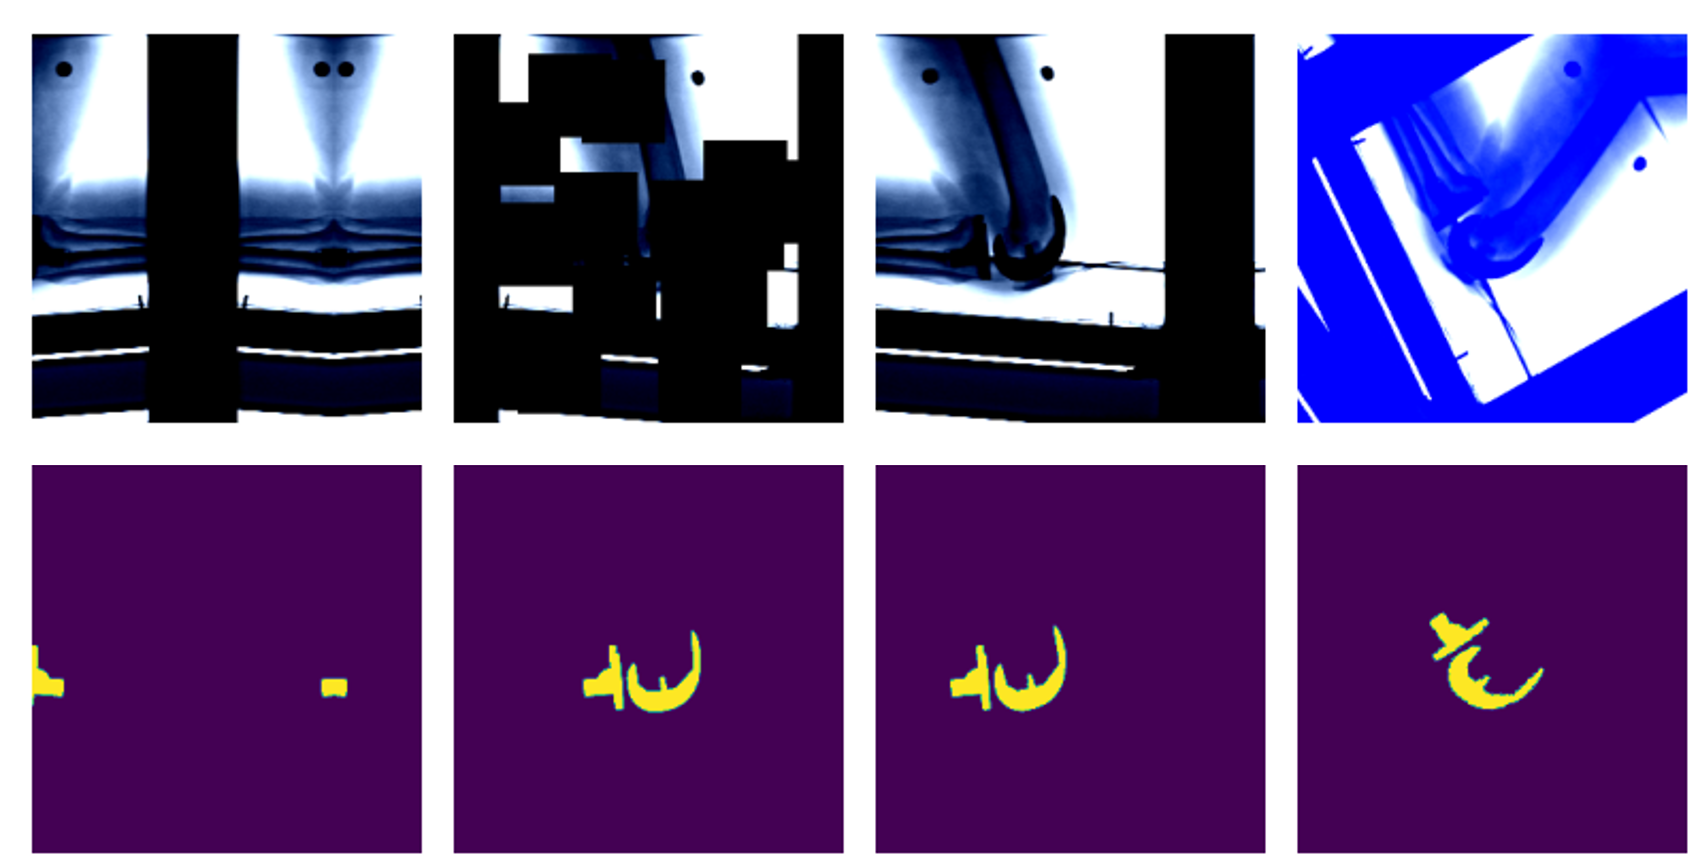
\includegraphics[width=.9\linewidth]{/home/ajensen123@ad.ufl.edu/repo/lit-review/figures/raster/augmentations.png}
\end{center}
\end{frame}
\begin{frame}[label={sec:org6141ee9}]{Normalized Fourier Descriptor Shape Libraries}
\begin{columns}
\begin{column}{0.37\columnwidth}
\begin{itemize}
\item Pose initialization using segmentation output.
\item \(\pm 30^{\circ}\) library span at \(3^{\circ}\) increments.
\end{itemize}
\end{column}
\begin{column}{0.7\columnwidth}
\begin{center}
\includegraphics[width=2in]{/home/ajensen123@ad.ufl.edu/repo/lit-review/figures/raster/banks-nfd-library.png}
\end{center}
\begin{center}
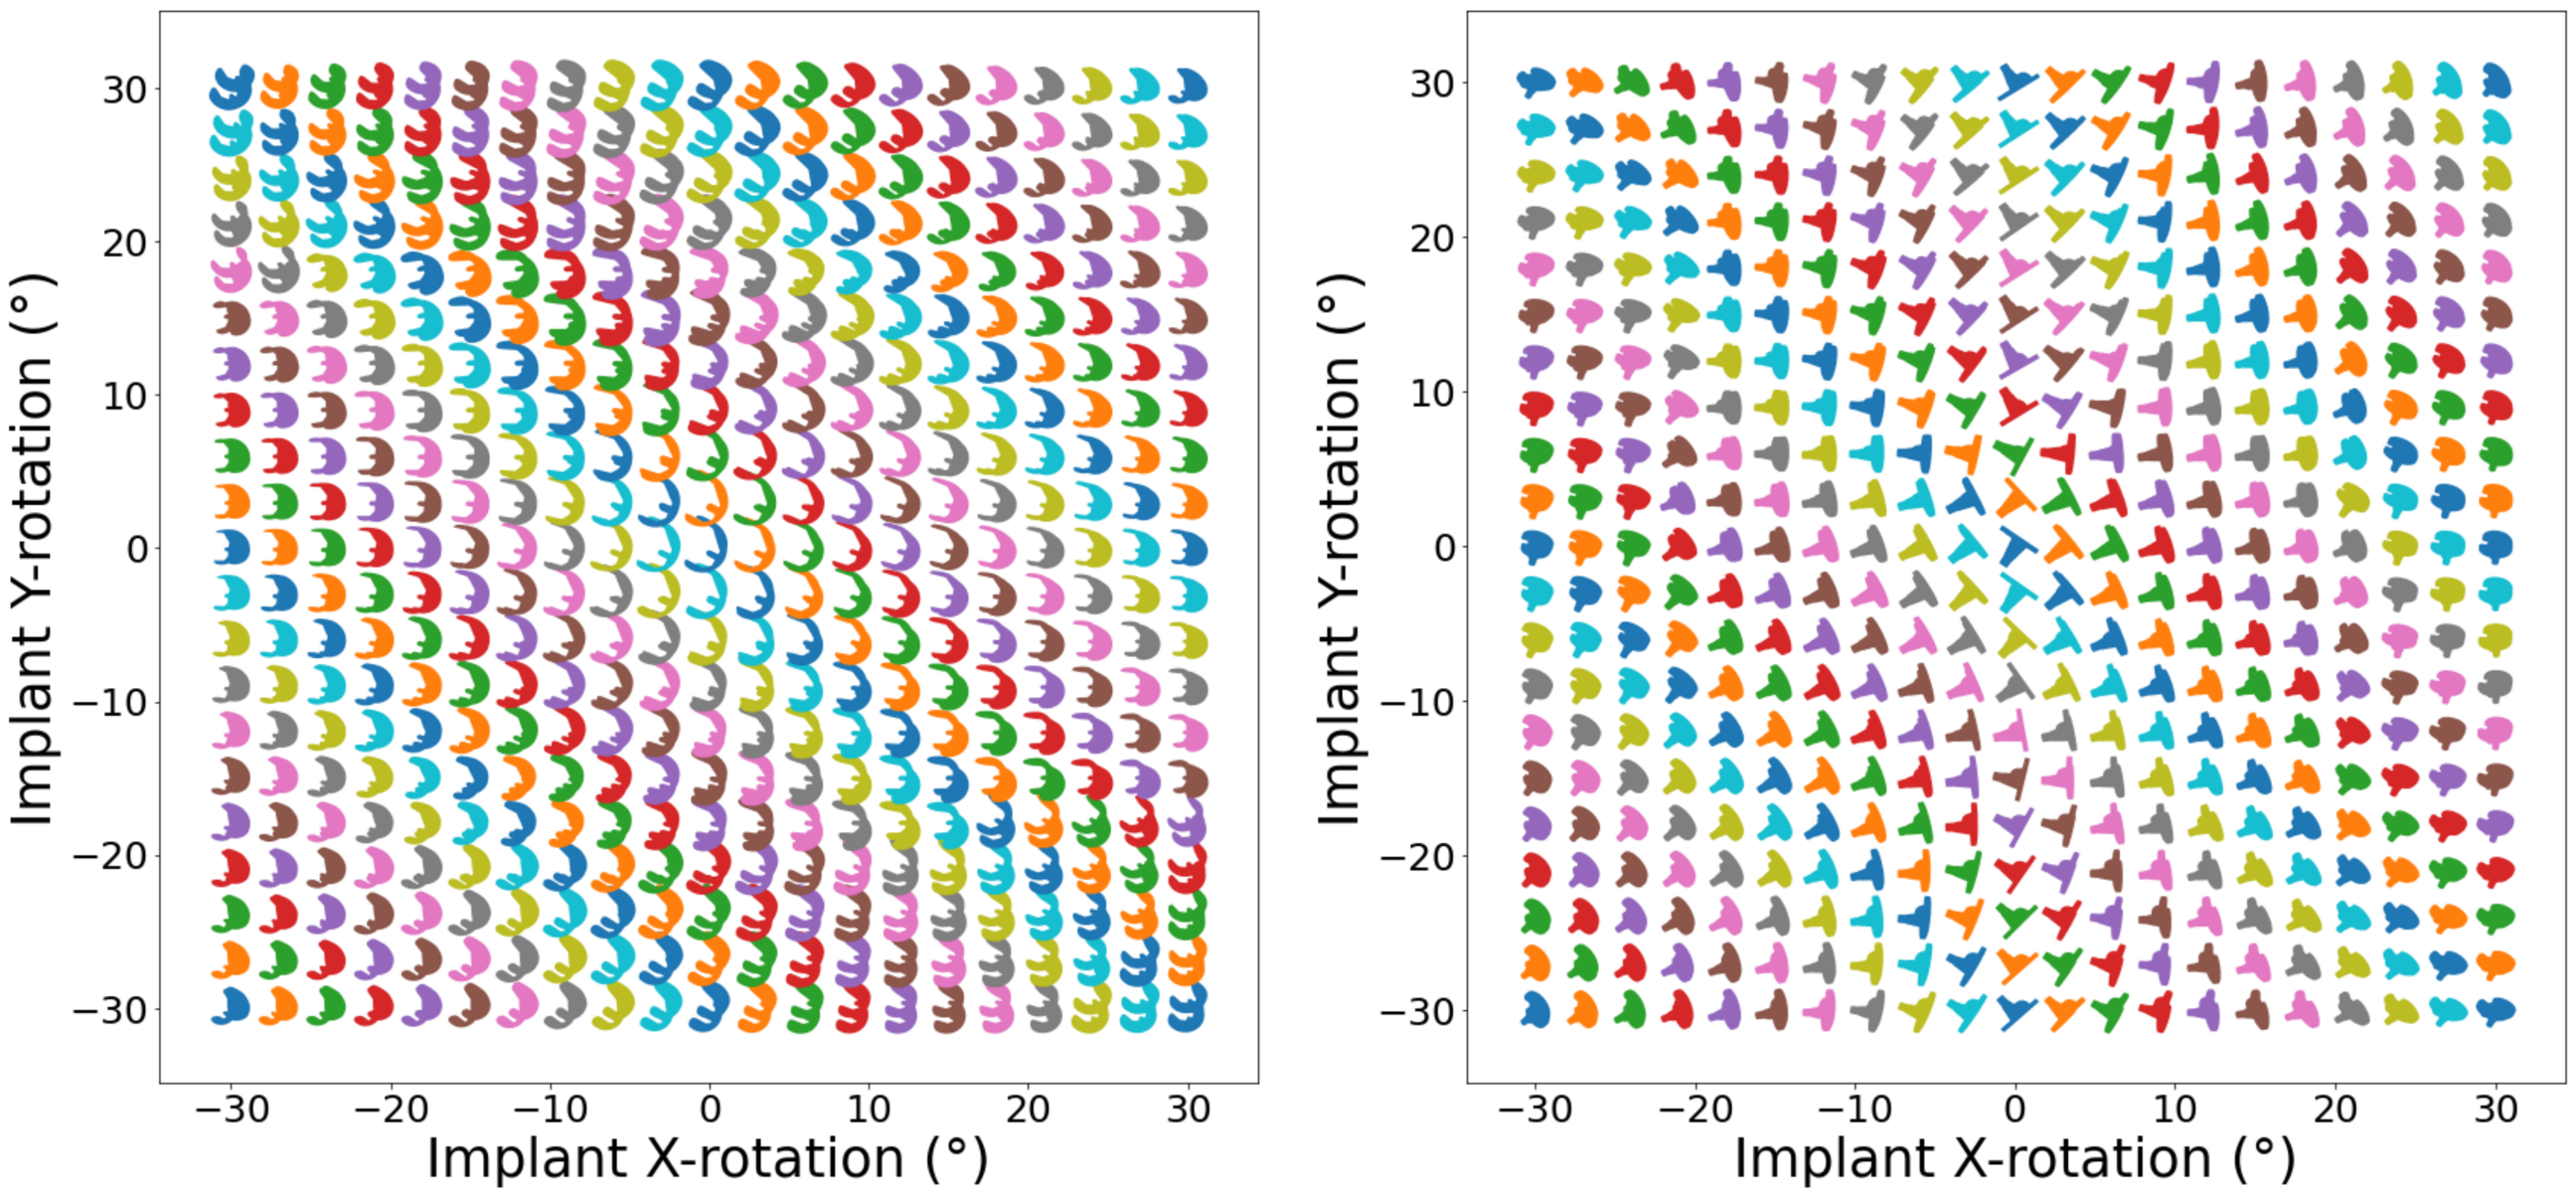
\includegraphics[width=3.25in]{/home/ajensen123@ad.ufl.edu/repo/lit-review/figures/raster/jtml-nfd.png}
\end{center}
\end{column}
\end{columns}
\end{frame}
\begin{frame}[label={sec:org07f0891}]{Pose Refinement Using Global Optimization}
\begin{columns}
\begin{column}{0.5\columnwidth}
\begin{itemize}
\item Two main features
\begin{itemize}
\item Objective function
\item Optimization routine
\end{itemize}
\end{itemize}
\end{column}
\begin{column}{0.5\columnwidth}
\begin{equation*}
    \argmin_{x}\{f(x) : x \in \Omega\}
\end{equation*}
\end{column}
\end{columns}
\end{frame}
\begin{frame}[label={sec:org783b51b}]{Contour-based Objective Function}
\begin{columns}
\begin{column}{0.5\columnwidth}
\begin{itemize}
\item With accurate projection, contours provide a strong heuristic for orientation.
\item Overlapping pixels between CNN segmentation and projected implant.
\begin{itemize}
\item \(L_1\) norm has quick parallel computation.
\end{itemize}
\end{itemize}

\begin{equation*}
  J = \sum_{i \in H}\sum_{j \in W}|I_{ij} - P_{ij}| = L_{1}(I,P)
\end{equation*}

\begin{itemize}
\item Sensitive to minor perturbations
\end{itemize}
\end{column}
\begin{column}{0.6\columnwidth}
\begin{center}
\includegraphics[width=.9\linewidth]{/home/ajensen123@ad.ufl.edu/repo/lit-review/figures/raster/registered-tka.png}
\end{center}
\end{column}
\end{columns}
\end{frame}
\begin{frame}[label={sec:org8a0773c}]{Improving Robustness}
\begin{columns}
\begin{column}{0.5\columnwidth}
\begin{itemize}
\item Dilation decreases sensitivity to perturbations.
\item Multi-stage optimization can reduce dilation back to original edges.
\end{itemize}
\end{column}
\begin{column}{0.6\columnwidth}
\begin{center}
\includegraphics[width=\textwidth]{/home/ajensen123@ad.ufl.edu/repo/lit-review/figures/raster/flood-dilated-contour.png}
\end{center}
\end{column}
\end{columns}
\end{frame}
\begin{frame}[label={sec:org5047e6f}]{Optimization Routine}
\begin{itemize}
\item No analytic form of the objective function exists, it \alert{\alert{must}} be sampled at points of interest.
\begin{itemize}
\item Black Box Optimization \autocites{audetDerivativeFreeBlackboxOptimization2017}[][]{bajajBlackBoxOptimizationMethods2021}
\end{itemize}
\end{itemize}
\end{frame}
\begin{frame}[label={sec:orga5997f0}]{Lipschitzian Optimization}
\begin{columns}
\begin{column}{0.5\columnwidth}
\begin{itemize}
\item Robust, global, black-box optimization routine if Lipschitz constant (\(K\)) is known \autocite{shubertSequentialMethodSeeking1972}.
\item Lipschitz constant bounds the rate of change of a function.
\item What if you don't know the Lipschitz constant?
\end{itemize}
\end{column}
\begin{column}{0.6\columnwidth}
\begin{center}
\includegraphics[width=2in]{/home/ajensen123@ad.ufl.edu/repo/lit-review/figures/raster/shubert-step1.png}
\end{center}
\begin{center}
\includegraphics[width=2in]{/home/ajensen123@ad.ufl.edu/repo/lit-review/figures/raster/shubert-step2.png}
\end{center}
\begin{center}
\includegraphics[width=2in]{/home/ajensen123@ad.ufl.edu/repo/lit-review/figures/raster/shubert-step3.png}
\end{center}
\end{column}
\end{columns}
\end{frame}
\begin{frame}[label={sec:org489eb92}]{Lipschitzian Optimization without the Lipschitz Constant}
\begin{center}
\includegraphics[width=2.5in]{/home/ajensen123@ad.ufl.edu/repo/lit-review/figures/raster/jones-direct-title.png}
\end{center}
\begin{itemize}
\item Sample end-points instead of intersecting lines.
\item Potentially optimal regions based on value at center and total size.
\begin{itemize}
\item Trisect potentially optimal regions and re-sample centers
\end{itemize}
\end{itemize}
\begin{center}
\includegraphics[width=2.5in]{/home/ajensen123@ad.ufl.edu/repo/lit-review/figures/raster/direct-1D.png}
\end{center}
\end{frame}
\begin{frame}[label={sec:org12e9404}]{Trisecting Region}
\begin{columns}
\begin{column}{0.4\columnwidth}
\begin{equation*}
  \begin{bmatrix}
    f(x=c_{1}) & d(c_{1})\\
    f(x=c_{2}) & d(c_{2})\\
    \vdots & \vdots \\
    f(x=c_{N}) & d(c_{N})
  \end{bmatrix}
\end{equation*}
Where

\begin{align*}
  f(x=c_{i}) &\equiv \text{Sampled function value} \\
  d(c_{i}) & \equiv \text{ Sub-domain size } \\
  & \text{ for } i \in [1,N]
\end{align*}
\end{column}
\begin{column}{0.6\columnwidth}
\begin{center}
\includegraphics[width=\textwidth]{/home/ajensen123@ad.ufl.edu/repo/lit-review/figures/raster/direct-1D-stage1.png}
\end{center}
\end{column}
\end{columns}
\end{frame}
\begin{frame}[label={sec:org7bf8266}]{Another Iteration}
\begin{columns}
\begin{column}{0.4\columnwidth}
\begin{equation*}
  \begin{bmatrix}
    f(x=c_{1}) & d(c_{1})\\
    f(x=c_{2}) & d(c_{2})\\
    \vdots & \vdots \\
    f(x=c_{N}) & d(c_{N})
  \end{bmatrix}
\end{equation*}
Where

\begin{align*}
  f(x=c_{i}) &\equiv \text{Sampled function value} \\
  d(c_{i}) & \equiv \text{ Sub-domain size } \\
  & \text{ for } i \in [1,N]
\end{align*}
\end{column}
\begin{column}{0.6\columnwidth}
\begin{center}
\includegraphics[width=\textwidth]{/home/ajensen123@ad.ufl.edu/repo/lit-review/figures/raster/direct-1D-stage2.png}
\end{center}
\end{column}
\end{columns}
\end{frame}
\begin{frame}[label={sec:org51b0ee7}]{Determining Potentially Optimal Regions}
\begin{itemize}
\item Convex hull \autocites{grahamEfficientAlgorithDetermining1972}[][]{jarvisIdentificationConvexHull1973}[][]{chanOptimalOutputsensitiveConvex1996}[][]{barberQuickhullAlgorithmConvex1996} of region size vs. center value
\end{itemize}

\begin{center}
\includegraphics[width=0.6\textwidth]{/home/ajensen123@ad.ufl.edu/repo/lit-review/figures/raster/direct-convex-hull.png}
\end{center}
\end{frame}
\begin{frame}[label={sec:orgf95978d}]{DiRECT for Joint Track Machine Learning}
\begin{itemize}
\item Search region is along all 6 degrees of freedom.
\begin{itemize}
\item Normalize to \([0,1]\).
\end{itemize}
\item Three stages, each with decreasing levels of dilation.
\begin{itemize}
\item Iteration budget for each stage.
\end{itemize}
\end{itemize}
\begin{center}
\begin{tabular}{lllr}
Stage & Budget [Iterations] & Search Range [mm,deg] & Dilation (pixels)\\
\hline
``Tree'' & \textasciitilde{}20,000 & \(\pm 45\) & 5\\
``Branch'' & \textasciitilde{}20,000 & \(\pm 25\) & 3\\
``Leaf'' & \textasciitilde{}10,000 & \(\pm 100\) \((z_{trans})\) / \(\pm 3\) \((else)\) & 1\\
\end{tabular}
\end{center}
\end{frame}
\begin{frame}[label={sec:org6f0d1d3}]{Testing Performance}
Now that we have our refined poses, how well does out system perform?
\begin{center}
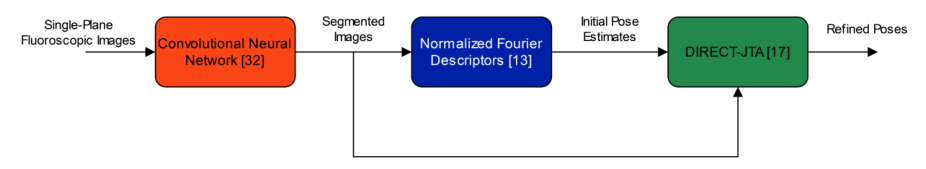
\includegraphics[width=\textwidth]{/home/ajensen123@ad.ufl.edu/repo/lit-review/figures/raster/jtml-pipeline.png}
\end{center}
\end{frame}
\begin{frame}[label={sec:orgb52089a}]{Validation}
\begin{itemize}
\item Independent research group using Model-Based RSA.
\item Determine the level of concordance between the two measurement systems
\begin{itemize}
\item Bland-Altmann Plots
\end{itemize}
\item Achieved clinically acceptable accuracy \autocites{brobergValidationMachineLearning2023}[][]{jensenJointTrackMachine2023}.
\item Highly repeatable
\end{itemize}

\begin{center}
\includegraphics[width=0.7\textwidth]{/home/ajensen123@ad.ufl.edu/repo/lit-review/figures/raster/broberg-bland-altmann.png}
\end{center}
\end{frame}
\begin{frame}[label={sec:org6349466}]{Awards}
The work presented in this aim won the HAP Paul Award for Best Paper from the International Society for Technology in Arthroplasty's 2022 Annual Meeting.
\begin{center}
\includegraphics[width=0.7\textwidth]{/home/ajensen123@ad.ufl.edu/repo/lit-review/figures/raster/ista-hap-paul-talk.png}
\end{center}
\end{frame}
\subsection{Aim 2 - Correcting Symmetric Implant Ambiguity}
\label{sec:org9739017}
\begin{frame}[label={sec:orgf5805fb}]{Goal}
\begin{itemize}
\item The goal of this aim is to validate and test methods that can overcome single-plane limitations for model-image registration.
\begin{itemize}
\item Out-of-plane (OOP) Translation
\item Symmetry Traps
\end{itemize}
\end{itemize}
\end{frame}
\begin{frame}[label={sec:orgeb44edd}]{Translation}
\begin{itemize}
\item Depth perception is lost when using a single camera.
\item Utilize a virtual ``spring'' to constrain relative OOP translation between implant components.
\end{itemize}

\begin{equation*}
  J = \alpha L_{1}(I,P) + \beta ML(Fem,Tib)
\end{equation*}

Where
\begin{equation*}
  ML \equiv \text{ Relative mediolateral translation }
\end{equation*}
\end{frame}
\begin{frame}[label={sec:orge09b344}]{Symmetry Traps}
\begin{columns}
\begin{column}{0.5\columnwidth}
With a symmetric tibial implant, the contour is not always a perfect heuristic for true pose.

Found ``ambiguous zone'' within \(3^{\circ}\) of pure lateral pose with high propensity for symmetry traps \autocite{jensenJointTrackMachine2023}.
\end{column}
\begin{column}{0.6\columnwidth}
\begin{center}
\includegraphics[width=\textwidth]{/home/ajensen123@ad.ufl.edu/figures/raster/sym-trap-quadrants-no-captions.png}
\end{center}
\end{column}
\end{columns}
\end{frame}
\begin{frame}[label={sec:org44c8255}]{Solving the Symmetric Pose}
\begin{columns}
\begin{column}{0.55\columnwidth}
Algorithm devised to ``flip'' pose into symmetric counterpart.
\begin{enumerate}
\item Determine viewing ray from camera to implant centroid, denote \(\vec{v}\), normalize.
\item Denote symmetric-plane normal vector \(\vec{s}\), normalize.
\item Measure relative ``off-lateral'' orientation of implant, \(\cos(\theta) = \dfrac{\vec{v} \cdot \vec{s}}{||\vec{v} || ||\vec{s} || }\)
\item Apply body-centered rotation to implant about \(\vec{m} = \vec{s} \times \vec{v}\) by \(\psi = 2\theta\).
\end{enumerate}
\end{column}
\begin{column}{0.5\columnwidth}
\begin{center}
\includegraphics[width=0.75\textwidth]{/home/ajensen123@ad.ufl.edu/figures/raster/symmetry_flipper.png}
\end{center}
\end{column}
\end{columns}
\end{frame}
\begin{frame}[label={sec:org1cbdc00}]{Methods - Training Set}
\begin{columns}
\begin{column}{0.5\columnwidth}
\begin{itemize}
\item ``Symmetric'' poses for each of the 12,000 frames were calculated using the ``flipper'' algorithm, yielding \textasciitilde{}24,000 total training samples.

The input for each sample was \([\theta_{F/E}, \theta_{V/V}, \theta_{I/E}, \psi]\), and the output was one of \(\{\text{True}, \text{Symmetric}\}\)
\end{itemize}
\end{column}
\begin{column}{0.5\columnwidth}
\begin{figure}[htbp]
\centering
\includegraphics[width=\textwidth]{/home/ajensen123@ad.ufl.edu/figures/raster/symmetry-trap-dataset.png}
\caption{The training data plotted with each axis representing an anatomical rotation (origin not to scale).}
\end{figure}
\end{column}
\end{columns}
\end{frame}
\begin{frame}[label={sec:org1a8af2c}]{Methods - Machine Learning}
Using \texttt{scikit-learn}, the following classifiers were implemented:

\begin{itemize}
\item Support Vector Machine, K-Nearest-Neighbors, AdaBoost, Histogram Gradient Boosting, Bagging Estimator, Stacked Generalization, Majority Voting Classifier
\end{itemize}
\end{frame}
\begin{frame}[label={sec:org7a6f44c},fragile]{Methods - Fixing ``Symmetry Traps''}
 For an input image sequence, the following is performed:

\begin{enumerate}
\item Each pose and its symmetric counterpart are fed into the machine learning classifier
\begin{enumerate}
\item If the outputs are different, take the pose labeled ``true'' as the correct pose.
\item If the outputs are the same, (i.e. both a pose and its symmetric counterpart return ``true''), label image ``ambiguous''
\end{enumerate}
\item For all images that are \texttt{NOT} ambiguous, construct a cubic spline through the three rotation measurements.
\item For all images that are labeled ``ambiguous'', determine which of the two poses is closer to the spline, and take that as the ``correct'' pose.
\end{enumerate}
\end{frame}
\begin{frame}[label={sec:org0e92922}]{Results - ML Classification}
\begin{center}
\includegraphics[width=\textwidth]{/home/ajensen123@ad.ufl.edu/figures/raster/sym-trap-ML-table.png}
\end{center}
\end{frame}
\begin{frame}[label={sec:orgb401a1b}]{Results - Fixing ``Symmetry Traps''}
\begin{itemize}
\item Accuracy: 91.9\%
\item Sensitivity: 0.674
\item Specificity: 0.940
\end{itemize}

The distribution of \(\psi\) for correct and incorrect frames was measured.
\begin{itemize}
\item Average \(\psi_{correct}=16.6^{\circ}\).
\item Average \(\psi_{incorrect} = 7.12^{\circ}\).
\end{itemize}
\end{frame}
\begin{frame}[label={sec:org1307aed}]{Results - Stratified \(\psi\) Correction Performance}
\begin{center}
\includegraphics[width=\textwidth]{/home/ajensen123@ad.ufl.edu/figures/raster/stratified-psi-ML-table.png}
\end{center}
\end{frame}
\begin{frame}[label={sec:org6a6cd19}]{Discussion}
\begin{itemize}
\item Reliable post-processing method to overcome pernicious issue (30 years in the making!)
\item Suggests an imaging setup for measuring kinematics slightly off-oblique to escape ``ambiguous zone''
\end{itemize}
\end{frame}
\subsection{Aim 3 - Musings on a ``Kinematics Translator'' and Synthetic Kinematics Data}
\label{sec:org15e62c2}
\subsection{Aim 4 - This will definitely work on shoulders, right?}
\label{sec:orgc7b8d19}

\begin{frame}[label={sec:org050c458}]{Spoiler Alert}
\begin{columns}
\begin{column}{0.3\columnwidth}
No, it won't.
\end{column}
\begin{column}{0.7\columnwidth}
\begin{center}
\includegraphics[width=1.5in]{/home/ajensen123@ad.ufl.edu/figures/raster/BAD_IE_HUM.png}
\end{center}

\begin{center}
\includegraphics[width=1.5in]{/home/ajensen123@ad.ufl.edu/figures/raster/BAD_PROXDIST_HUM.png}
\end{center}
\end{column}
\end{columns}
\end{frame}
\begin{frame}[label={sec:org271cf16}]{Goal}
Establish a protocol for exploring the relative sensitivity of input orientation to projected shape
\end{frame}
\begin{frame}[label={sec:org0ed54af}]{JTML on Shoulders}
\begin{table}[h!]
\small
	\caption{Root mean squared differences between JointTrack Machine Learning optimized kinematics and manually registered kinematics on single-plane fluoroscopy} \label{tab:jtml-tsa-tka-vals}
	\begin{tabularx}{\linewidth}{ccccccc}\hline
		 Implant Type & $x_{trans} (mm)$ & $y_{trans} (mm)$ & $z_{trans} (mm)$ & $x_{rot} (^{\circ})$ & $y_{rot} (^{\circ})$ & $z_{rot} (^{\circ})$ \\ \hline
		Humeral            & 8.46             & 8.64             & 152.78           & 22.59                & 64.74                & 11.81                \\
		Glenosphere        & 0.97             & 1.44             & 32.58            & 13.72                & 26.40                & 8.30                 \\
		Femoral            & 0.57             & 0.39             & 26.95            & 0.66                 & 0.73                 & 0.60                 \\
		Tibial             & 0.67             & 0.64             & 27.17            & 1.63                 & 2.74                 & 0.66                 \\\hline
	\end{tabularx}
\end{table}
\end{frame}
\begin{frame}[label={sec:org61799f6}]{Modified Mean Surface Distance}
\begin{itemize}
\item In order to improve error gradient, a modified mean surface distance was incorporated into the cost function.
\item The mean of the dot product between the projection estimate and a distance map of the CNN segmentation.
\end{itemize}
\begin{equation}
  \label{eq:DMCF}
  J = \dfrac{Proj \cdot DM}{\sum Proj}
\end{equation}
\end{frame}
\begin{frame}[label={sec:org41dcc69}]{Modified Asymmetric Keypoint Distance}
\begin{itemize}
\item Early psychological research deemed curvature as highly salient for object recognition \autocites{attneaveInformationalAspectsVisual1954}[][]{attneaveQuantitativeStudyShape1956}. This aimed to place additional emphasis on autonomously selected high-curvature regions.
\begin{itemize}
\item Extracted regions of high-curvature using Menger's Algorithm \autocite{legerMengerCurvatureRectifiability1999}.
\item Utilized a modified asymmetric surface distance on the discrete set of keypoints.
\end{itemize}
\end{itemize}

\begin{equation}
  \label{eq:curv-keypoint}
  \begin{split}
    \displaystyle J &= \dfrac{\sum_{k \in \mathbb{K}}(\min_{p\in Proj}(p \cdot DM_{k}))}{N_k} \\
      &\text{where}\\
    \mathbb{K} &= \text{Set of all keypoints} \\
    DM_{k} &= \text{Distance map for keypoint $k$} \\
  \end{split}
\end{equation}
\end{frame}
\begin{frame}[label={sec:org3faff67}]{2-Dimensional Shape}
\end{frame}
\begin{frame}[label={sec:org7fea3aa}]{Invariant Angular Radial Transform Descriptor}
The Invariant Angular Radial Transform provides an orthogonal spatial basis function to describe binary images.

\begin{figure}[htbp]
\centering
\includegraphics[width=0.7\textwidth]{/home/ajensen123@ad.ufl.edu/figures/raster/ART_basis.png}
\caption{The basis ``vectors'' for the invariant angular radial transform. From \autocite{leeNewShapeDescription2012}.}
\end{figure}
\end{frame}
\begin{frame}[label={sec:org9e15a51}]{IARTD Feature Vector}
The complez feature vector for IARTD is constructed to ensure orthogonality and rotational invariance for the magnitude. Prior to calculation, the image coordinates are normalized such that \((0,0)\) is at the center, and each of the four corners are \((\pm 1, \pm 1)\).
\begin{equation}
  F_{np} = \int_{0}^{2\pi}\int_{0}^{1} f(\rho,\theta)V_{np}(\rho,\theta)\rho d\rho d\theta
\end{equation}


\begin{equation}
	\begin{split}
		f(\rho,\theta) & \equiv \text{ Input image in polar coordinates}  \\
		V_{np}(\rho,\theta)         & = \dfrac{1}{2\pi}e^{jp\theta}R_{n}(\rho)      \\
		R_{n}(\rho)    & =
		\begin{cases}
			1                   & n=0     \\
			2 \cos (\pi n \rho) & n \ne 0
		\end{cases}
	\end{split}
\end{equation}
\end{frame}
\begin{frame}[label={sec:org864d1d0}]{Normalizing IARTD Feature Vector}
We normalize the phase of the feature vector to ensure full rotational invariance.
\begin{equation}
  \begin{split}
    \phi'_{np} &= \phi_{np}-\phi_{n,1} \\
    F'_{np} &= F_{np}e^{-jp\phi_{n,1}}
  \end{split}
\end{equation}

The final feature vector is the constructed with the corrected phase and magnitude values. Values of \(p<2\) are redundant and removed per the original authors' suggestion \autocite{leeNewShapeDescription2012}.
\begin{equation}
  IARTD = \{|F'_{np}|,\phi'_{np}\} \text{ where } n\ge0,p\ge2
\end{equation}
\end{frame}
\begin{frame}[label={sec:orge763da3}]{Methods - Shape Difference}
\begin{columns}
\begin{column}{0.5\columnwidth}
The ``input shapes'' for each implant were the projected implants at \(\pm 30^{\circ}\) along each rotational axis at \(5^{\circ}\) increments.
\(1^{\circ}\) perturbations were applied along each rotation axis.

\begin{equation}
	\label{eq:shape-derivative}
	\begin{split}
		\Delta S(\delta)_{z,x,y}  \equiv & IARTD(R_{z,x,y,+\delta})                        \\
		                                 & - IARTD(R_{z,x,y,-\delta})                      \\
		\forall                          & \delta \in \{\delta_{x},\delta_{y},\delta_{z}\}
	\end{split}
\end{equation}
\end{column}
\begin{column}{0.5\columnwidth}
\begin{center}
\includegraphics[width=0.75\textwidth]{/home/ajensen123@ad.ufl.edu/figures/raster/rTSA_humeral_rotation_axes.png}
\end{center}
\end{column}
\end{columns}
\end{frame}
\begin{frame}[label={sec:org00305d4}]{Methods - Shape Sensitivity}
The \(\Delta S(\delta)_{z,x,y}\) vector is normalized to account for overall scale of each element, in-plane rotation inputs are averaged, and the 2-norm of the difference vector is defined as the shape sensitivity.

A larger vector would indicate that the shape changed more for that particular ``input shape'' and perturbation.

\begin{equation}
	\label{eq:z_rot_norm}
	\mathbb{S}(\delta)_{x,y} = \dfrac{\sum_{z} \| S(\delta)_{z,x,y} \|_{2}}{N}
\end{equation}
\end{frame}
\begin{frame}[label={sec:org6710cde}]{Results - Humeral Shape Sensitivity}
\begin{figure}[h!]
	\centering
	\includegraphics[width=0.3\linewidth]{~/figures/raster/Humeral_dx_sensitivity.png}
	\includegraphics[width=0.3\linewidth]{~/figures/raster/Humeral_dy_sensitivity.png}
	\includegraphics[width=0.3\linewidth]{~/figures/raster/Humeral_dz_sensitivity.png}
	\caption{The $\mathbb{S}$ plot for a humeral implant for $\delta$ rotations along the x, y, and z axis, respectively.}
	\label{fig:hum_sensitivity_plot}
\end{figure}
\end{frame}
\begin{frame}[label={sec:orgfc5f5f4}]{Results - Glenosphere Shape Sensitivity}
\begin{figure}[h!]
	\centering
	\includegraphics[width=0.3\linewidth]{~/figures/raster/Glenosphere_dx_sensitivity.png}
	\includegraphics[width=0.3\linewidth]{~/figures/raster/Glenosphere_dy_sensitivity.png}
	\includegraphics[width=0.3\linewidth]{~/figures/raster/Glenosphere_dz_sensitivity.png}
	\caption{The $\mathbb{S}$ plot for a glenosphere implant for $\delta$ rotations along the x, y, and z axis, respectively.}
	\label{fig:sca_sensitivity_plot}
\end{figure}
\end{frame}
\begin{frame}[label={sec:org8f37a3b}]{Results - Femoral Shape Sensitivity}
\begin{figure}[h!]
	\centering
	\includegraphics[width=0.3\linewidth]{~/figures/raster/Femoral_dx_sensitivity.png}
	\includegraphics[width=0.3\linewidth]{~/figures/raster/Femoral_dy_sensitivity.png}
	\includegraphics[width=0.3\linewidth]{~/figures/raster/Femoral_dz_sensitivity.png}
	\caption{The $\mathbb{S}$ plot for a femoral implant for $\delta$ rotations along the x, y, and z axis, respectively.}
	\label{fig:fem_sensitivity_plot}
\end{figure}
\end{frame}
\begin{frame}[label={sec:orgbe75d57}]{Results - Tibial Shape Sensitivity}
\begin{figure}[h!]
	\centering
	\includegraphics[width=0.3\linewidth]{~/figures/raster/Tibial_dx_sensitivity.png}
	\includegraphics[width=0.3\linewidth]{~/figures/raster/Tibial_dy_sensitivity.png}
	\includegraphics[width=0.3\linewidth]{~/figures/raster/Tibial_dz_sensitivity.png}
	\caption{The $\mathbb{S}$ plot for a tibial implant for $\delta$ rotations along the x, y, and z axis, respectively.}
	\label{fig:tib_sensitivity_plot}
\end{figure}
\end{frame}
\begin{frame}[label={sec:org97cb7b4}]{Key Takeaways}
\begin{itemize}
\item Humeral implant has the lowest \(\delta_y\) sensitivity of all implants, which is the difficult registration axis.
\item Tibial and glenosphere implants demonstrate a ``valley'' along rotation axis representing near-symmetry.
\begin{itemize}
\item For tibial implants, this is the axis most commonly associated with ``symmetry traps''.
\end{itemize}
\end{itemize}
\begin{figure}[h!]
	\centering
	\includegraphics[width=0.3\linewidth]{~/figures/raster/Glenosphere_dy_sensitivity.png}
	\includegraphics[width=0.3\linewidth]{~/figures/raster/Tibial_dy_sensitivity.png}
    \caption{Glenosphere (left) and tibial (right) $\delta_y$ shape sensitivities.}
\end{figure}
\end{frame}
\section{Conclusion}
\label{sec:org0282a99}
\begin{frame}[label={sec:org8fb5e6f}]{Conclusions}
Throughout the past four years, I have:
\begin{enumerate}
\item Established a fully autonomous method of measuring TKA kinematics from single plane fluoroscopy. This software is used globally by different research groups, and offers
\item Utilized machine learning to address ``symmetry traps'', an inherent limitation in single-plane TKA kinematics measurements for nearly 30 years. Additionally, we offer an alternative imaging protocol for accurately measuring TKA kinematics in a clinical setting.
\item Developed a pipeline for accessing the relative performance of autonomous registration for different implants, conclusively finding that implant geometry alone is not sufficient for every joint.
\end{enumerate}
\end{frame}
\begin{frame}[label={sec:orgb61f1c6},fragile, allowframebreaks, label=]{Presentations}
\begin{refsection}
  
\nocite{%
banksRegioneCaecorumRex2019,  daiComparativeAnalysisFixation2021, daiImpactFixationComponents2021, floodPracticalClinicalExamination2019, griffithAutomatedSegmentationGrading2022, jensenAutonomousMeasurement3D2022, jensenAutonomousMethodExtracting2021, jensenAutonomousMethodExtracting2021a, jensenComparisonClinicalComputational2020, jensenDeepLearningImage2023,  jensenRoutineClinicalExamination2020,jensenImpactSagittalResection2020}

  \printbibliography[title=Presentations]
\end{refsection}
\end{frame}
\begin{frame}[label={sec:org50f74e6},fragile, allowframebreaks, label=]{Publications}
\begin{refsection}
  
\nocite{%
brobergValidationMachineLearning2023, burtonAutomaticTrackingHealthy2021, jensenJointTrackMachine2022,
}

  \printbibliography[title=Publications]
\end{refsection}
\end{frame}
\begin{frame}[label={sec:org1c1f4e8}]{Timeline}
\begin{center}
\begin{tabular}{ll}
Date(s) & Event\\
\hline
2015-2019 & Mech. Eng. B.S, Magna Cum Laude, UF\\
April 2019 - April 2020 & Internship at Exactech\\
April 2020 & Started in Miller Lab\\
August 2020 & Officially Started PhD at UF\\
November 2021 & Best Presentation Award at ISTA: Emerging Technologies\\
April 2022 & Submitted JTML for HAP Paul Award\\
September 2022 & HAP Paul Award at ISTA 2022\\
November 2023 & Symmetry Trap Paper Submitted\\
December 2023 & Part-time Internship at Exactech Started\\
February 2024 & Revisions Requested for Symmetry Trap Paper\\
February 2024 & Implant Shape Sensitivity Paper Submitted\\
\end{tabular}
\end{center}
\end{frame}
\begin{frame}[label={sec:org5f2be39}]{Thank you!}
Thanks for listening!!
\end{frame}
\section{References}
\label{sec:org1e18e5b}
\begin{frame}[label={sec:org1648d81},fragile, allowframebreaks,  label=]{References}
\printbibliography
\end{frame}
\end{document}
